\section*{Overview} 

This tutorial will teach you how you
can create your own ICE Items via the built in tools within ICE.  To demonstrate
these tools, we will walk through the development of an ICE Item project for the
FERN code, a fast efficient nuclear reaction network solver. 

So we don't have to worry about building Fern for this tutorial, we have
provided a convenient Docker image for Fern that you may use.  
This image must be a part of your local docker daemon images list for use in
this tutorial. You can add the image to your local Docker daemon in 2 ways: build the
image with the provided Dockerfile, or load the image through the image tar ball we have provided. To
build it from scratch, in the same directory as the Dockerfile, run 
\begin{lstlisting}[language=bash,caption={bash version}]
docker build -t eclipseice/fern .
\end{lstlisting}
To load the image from the provided tar ball, run 
\begin{lstlisting}[language=bash,caption={bash version}]
docker load < fernImage.tar.gz
\end{lstlisting}

After creating a new ICE Item plugin project, we will demonstrate how to
provide a few lines of code to get a Model Item showing in ICE that creates
input files for FERN. After that we will add a little code to the FERN
JobLauncher to be able to execute FERN locally, remotely, or via the
provided Docker image. 

Before we begin, make sure you have ICE cloned (Developer $>$ ICE $>$ Clone ICE)
into your workspace, and the provided Docker image loaded to your local Docker daemon. 

\section*{Creating a New ICE Item Plugin Project}

\begin{figure}[h]
\centering
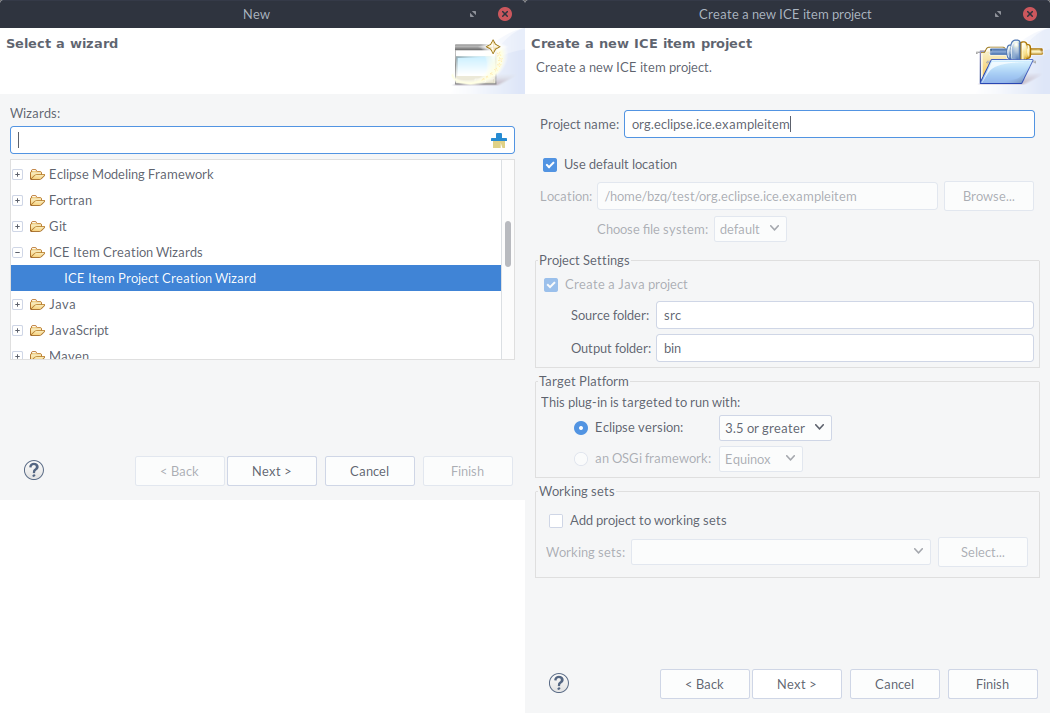
\includegraphics[width=\textwidth]{figures/comb12.png}
\label{fig:comb12}
\end{figure}

To create a new ICE Item project, navigate to \texttt{File $>$ New $>$ Other}
and open the \texttt{ICE Item Creation Wizards} folder and 
select \texttt{ICE Item Creation Wizard}. You will be met with a standard new
project wizard page, in which you can name your project.  We will call ours
\texttt{org.eclipse.ice.fern}. Once you have named your project click the \texttt{Next >} button.
\begin{center} 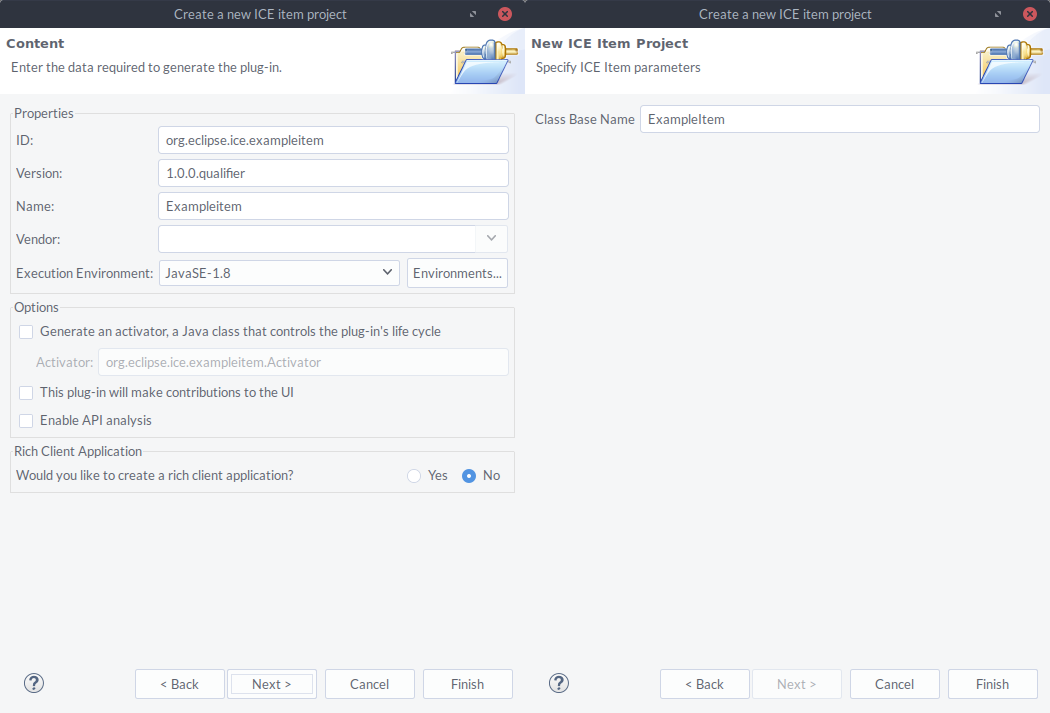
\includegraphics[width=\textwidth]{figures/comb23} \end{center}
Now you are able to customize the plugin-specific portions of the project. We do
not need an Activator to be generated, so uncheck that box, then select
\texttt{Next}. 

On this page you simply need to tell the wizard what you want to use as a base
name for your item classes.  We will call this one \texttt{Fern}. Then, we will
specify some information about how the item will handle input data.  Fern uses
the INI file format to specify data, so we will tell our item to use the built-in
functionality for INI files.  To do this  select \texttt{INI} from the \texttt{File Format} dropdown.  
Next we will provide a default data set to load when an item is created.  This step 
makes the item generation process much quicker by reducing the amount of code we need to write.
Click the \texttt{Browse} button and select the \texttt{alpha.ini} file from the data provided
in the tutorial files. 
When you have entered all of the required information you can
click the \texttt{Finish} button to generate your new ICE Item plugin project.

When the project has finished generating you should be able to explore the code
that has been created.  Within the source directory there will be two packages,
each containing two Java classes:

\begin{itemize} 
    \item \texttt{org.eclipse.ice.fern.launcher} 
    \begin{itemize}
        \item \texttt{FernLauncher.java} 
        \item \texttt{FernLauncherBuilder.java}
    \end{itemize} 
    \item \texttt{org.eclipse.ice.fern.model} 
    \begin{itemize} 
        \item \texttt{FernModel.java} 
        \item \texttt{FernModelBuilder.java}
    \end{itemize} 
\end{itemize}

To add functionality to the project you will only be responsible for editing
the \texttt{Launcher} and \texttt{Model} classes and can ignore the
\texttt{LauncherBuilder} and \texttt{ModelBuilder} classes.


\section*{Adding Functionality to the New Items}

\subsection*{The Fern Model}

The \texttt{FernModel} will be responsible for creating and
validating input parameters for FERN, in the form of a new FERN input file. 
The Fern Model is largely completed, thanks to the additional information about
the file format and initial data that we provided during the creation of the 
project.  

If you are interested in other ways that you can customize the model item you 
can open the \texttt{FernModel.java} and browse through the source code.  There
are comments that provide examples of other ways that the item can be set up 
and used.

\subsection*{Fern Launcher}
The Fern Launcher handles the actual execution of the FERN application. The
generator creates the FernLauncher as a subclass of ICE's JobLauncher, which
provides a large array of features and functionality. As a subclass of
JobLauncher, the FernLauncher enables users to execute Fern locally, remotely,
or even through a Docker image. To do so, we just need to add a small amount of
code that customizes the ICE job launching capabilities for Fern. 

The first bit of code to add to the FernLauncher specifies the name of the
actual Fern executable. In the setupItemInfo() method, set the execCommand to
the following: 
\begin{lstlisting}[language=Java]
execCommand = "${installDir}fern-exec";
\end{lstlisting}
This tells ICE that the Fern executable is called \texttt{fern-exec}, and to
set the overall execution command to it's install path plus the executable name.

As for the Hosts information in the setupForm() method, let's simply change the
install path to what we know it will be in the Docker container we will use -
\texttt{/usr/bin}.
You can actually just change this on the Fern Launcher UI, but for efficiency, let's
do it here. 
\begin{lstlisting}[language=Java]
addHost("localhost", "linux x86_64", "/usr/bin");
\end{lstlisting}
We also need to inform the JobLauncher what other files are involved in this
execution. To do that, the JobLauncher provides an addInputType() method. Add
the following to setupForm():
\begin{lstlisting}[language=Java]
addInputType("Network File", "networkFile", 
			"Network File Description", ".inp");
addInputType("Rate File", "rateFile", "
			Rate File Description", ".data");
\end{lstlisting}

And that should be it.
The generator has taken care of everything else for us.
We are now ready to launch ICE with our Fern plugin, and use the Fern Items we
have just created.

\section*{Using the New Fern Items}
Now, using these new Items is easy. Open the Run Configurations wizard with
\texttt{Run $>$ Run Configurations\ldots}, and open Eclipse Applications to see ICE
launch configurations for Mac, Linux, and Windows. Select the launch configuration for your OS and open the Plug-ins
tab. Scroll down to the \texttt{org.eclipse.ice.fern} plugin and turn it on for
this launch configuration by clicking the check box. Then click Apply and Run. 

With a new ICE instance open, close the Welcome view if necessary and go to
\texttt{File $>$ New $>$ Other} and select the Create Item Wizard. 
\begin{center} 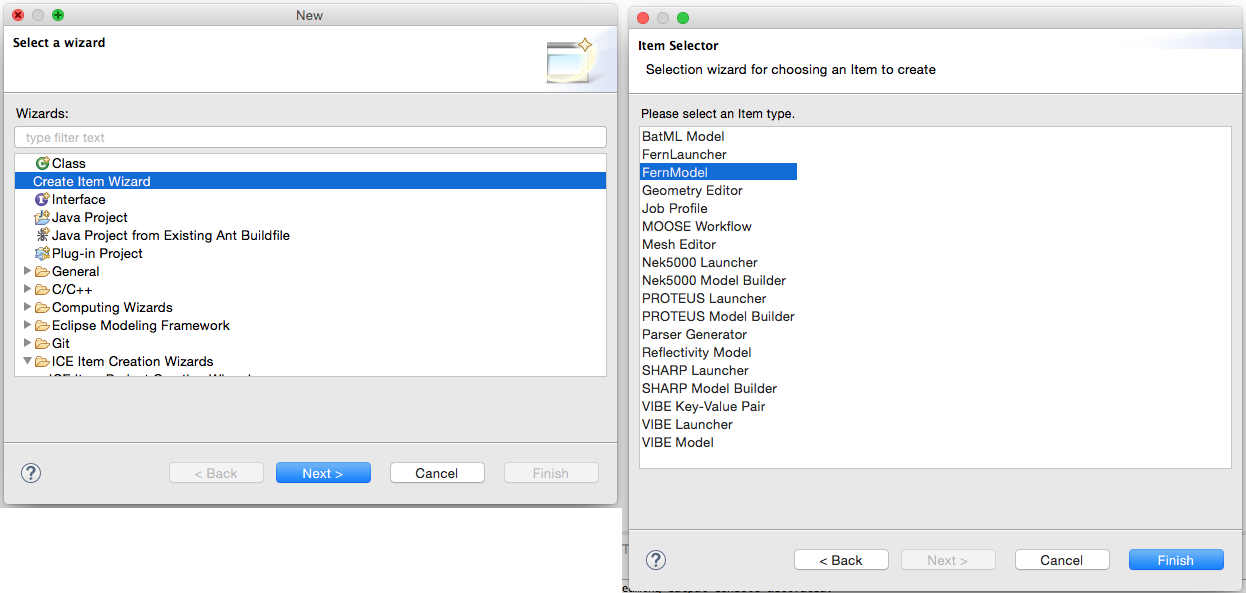
\includegraphics[width=\textwidth]{figures/creatingFernModelItem}
\end{center}
After selecting the FernModel Item, you will be presented with the view in the
figure below. 
\begin{center} 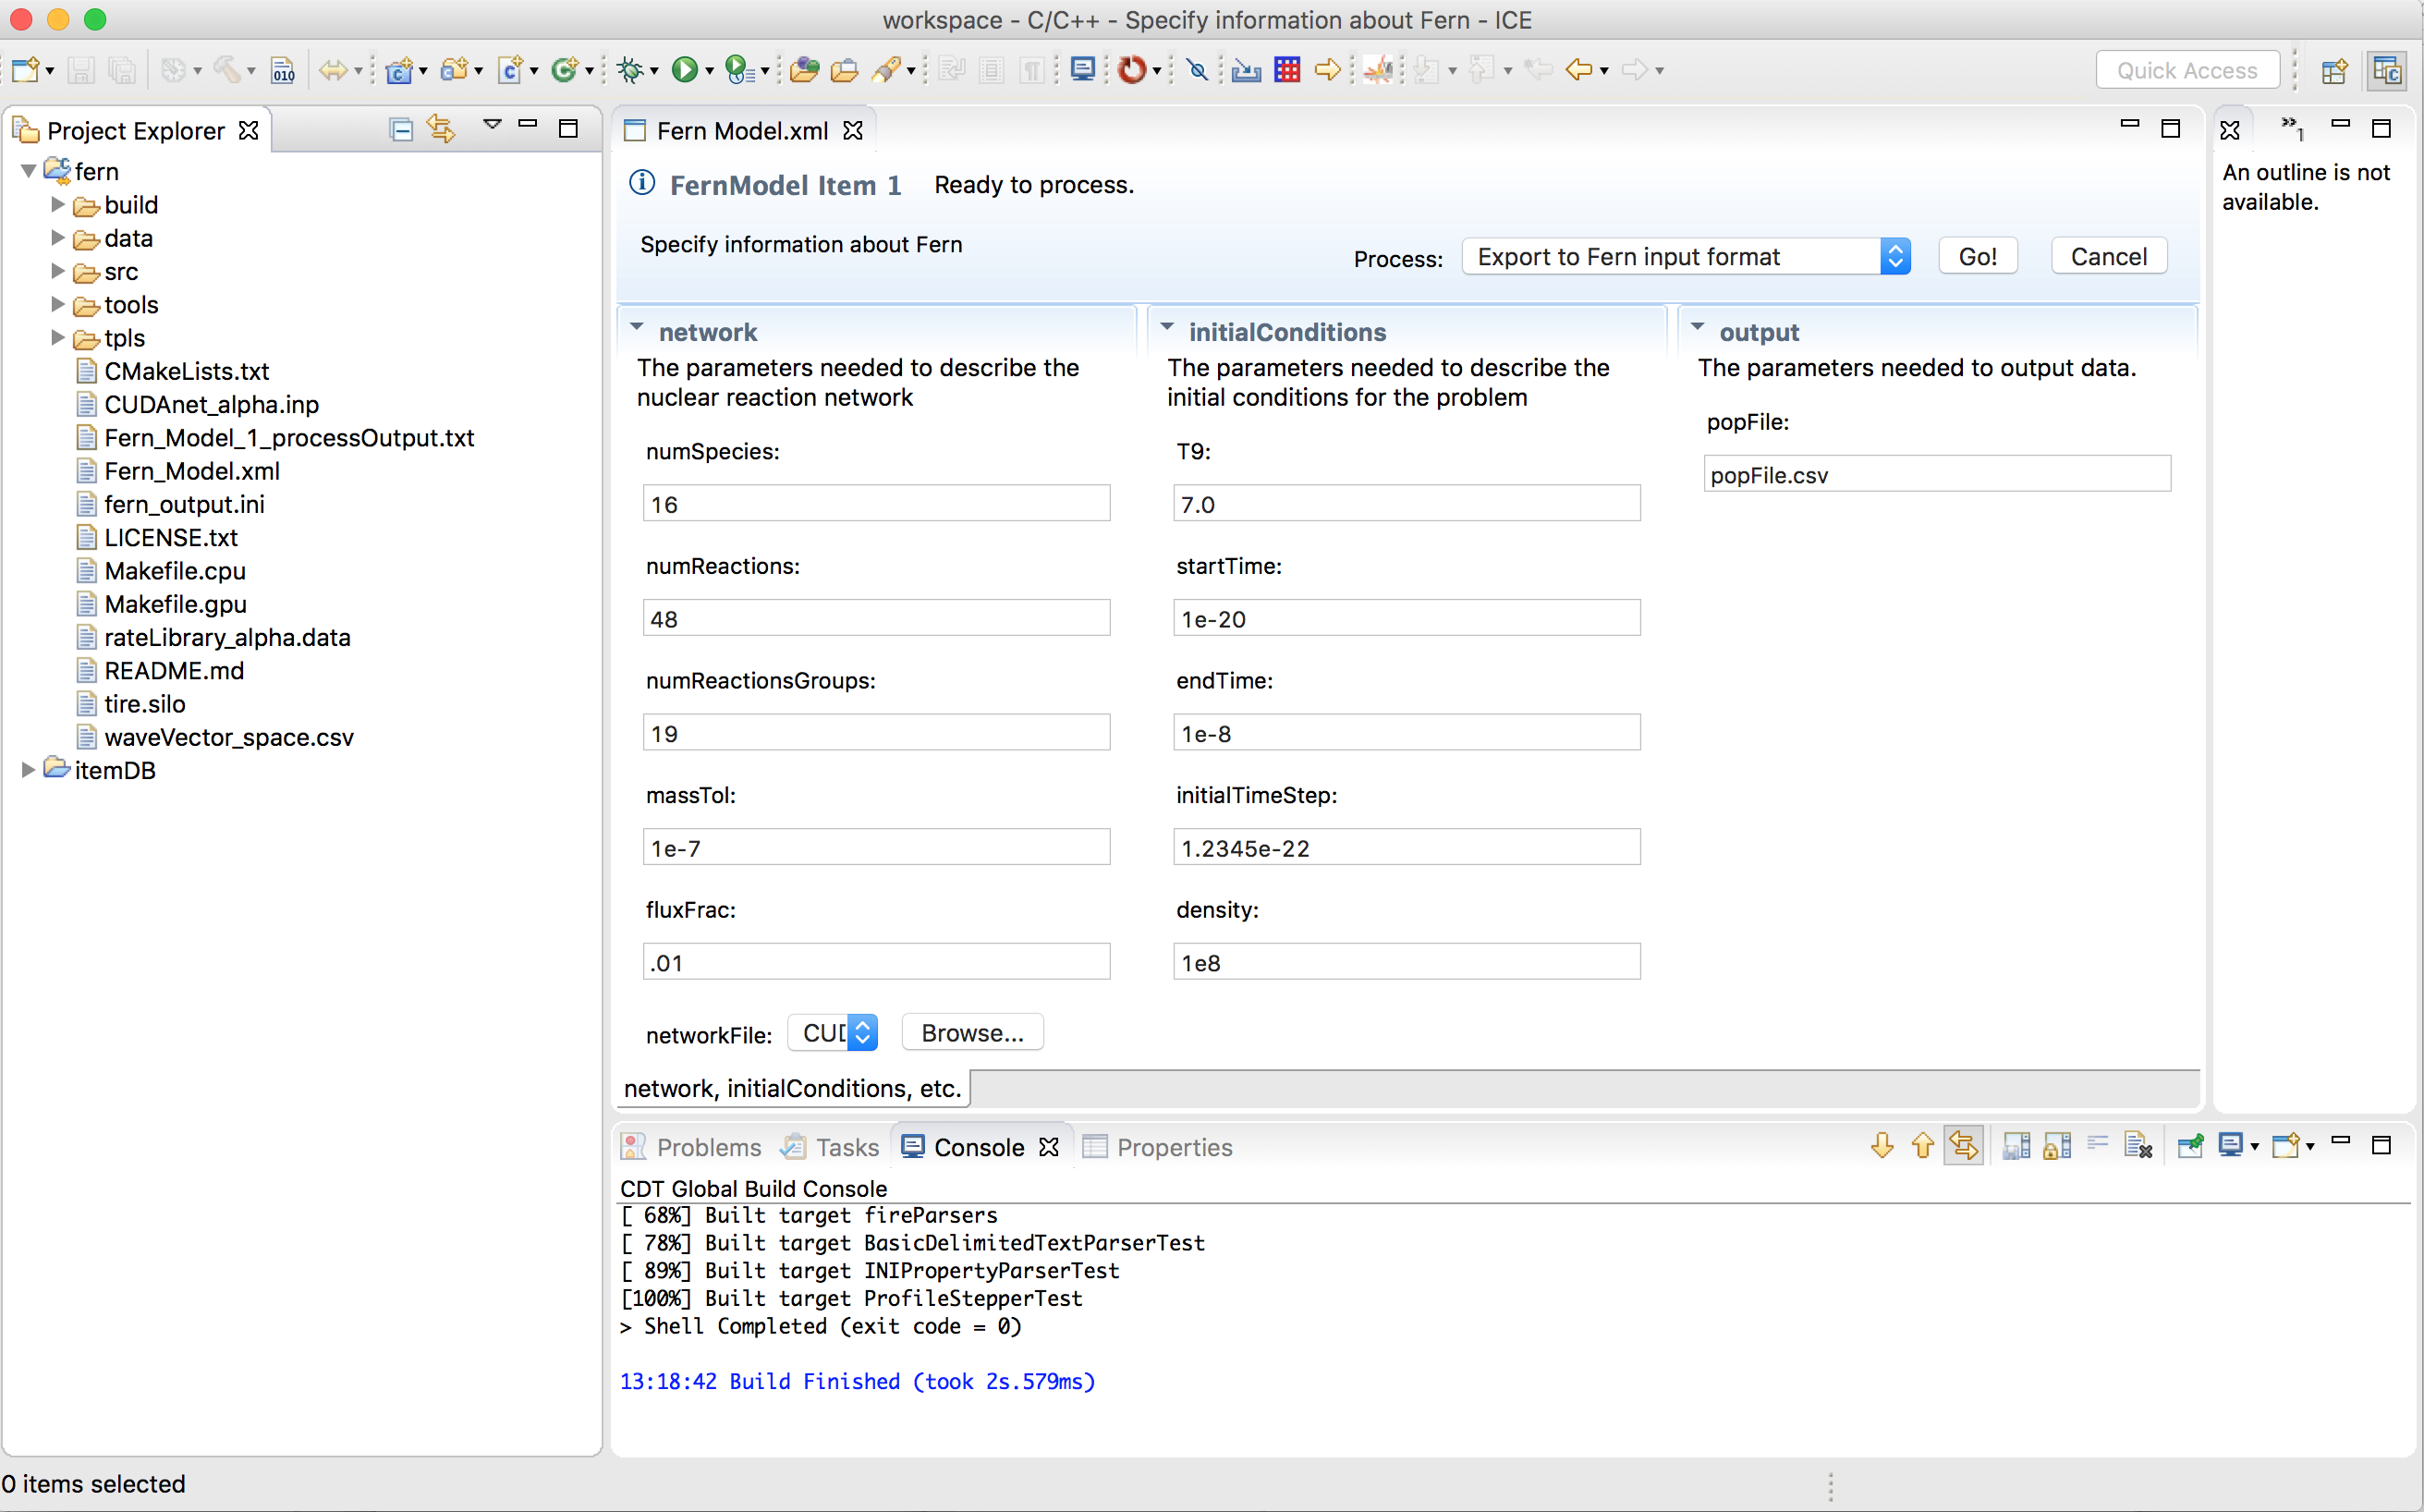
\includegraphics[width=\textwidth]{figures/fernmodelItem}
\end{center}
Here you can modify the various defaults with the values you would like for a
given Fern simulation. Once done, simply save the Item and click Go on the
Export to INI Process. This will execute the process of creating a new INI Fern
input file for use with the Fern Launcher. You can check the result by opening
the fern\_output.ini file, as shown below. 
\begin{center} 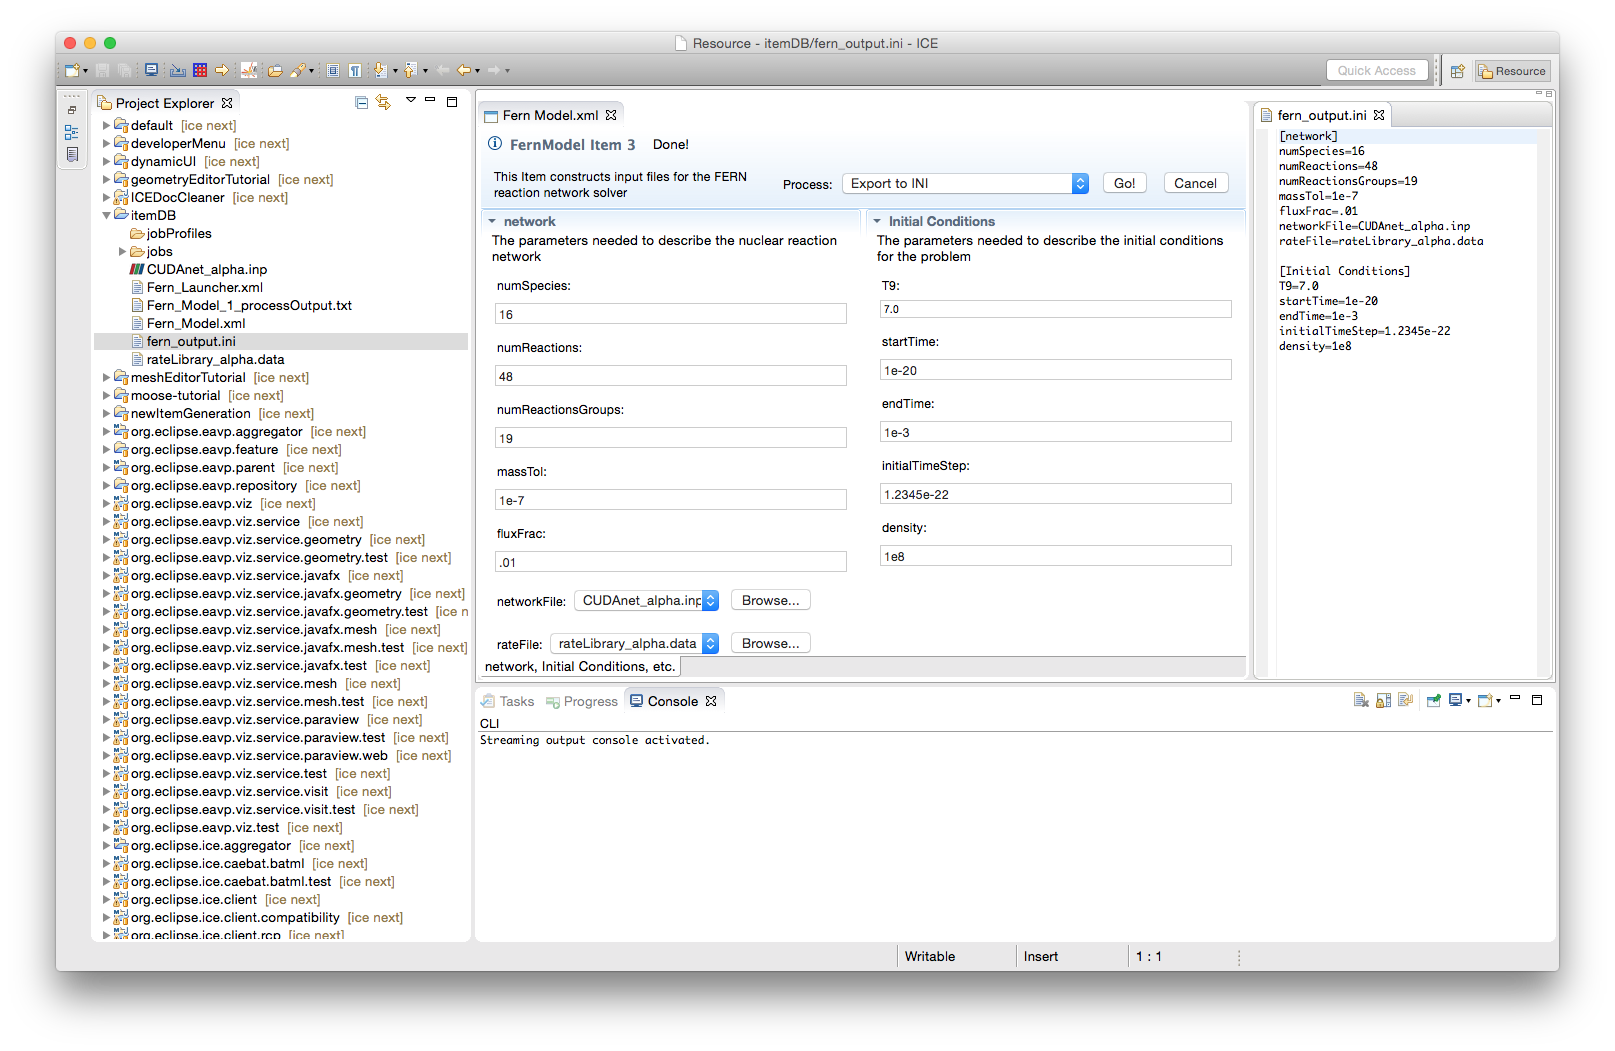
\includegraphics[width=\textwidth]{figures/result}
\end{center}

Now you can similarly create a new Fern Launcher. After creating the Launcher,
you should see a view like below. 
\begin{center} 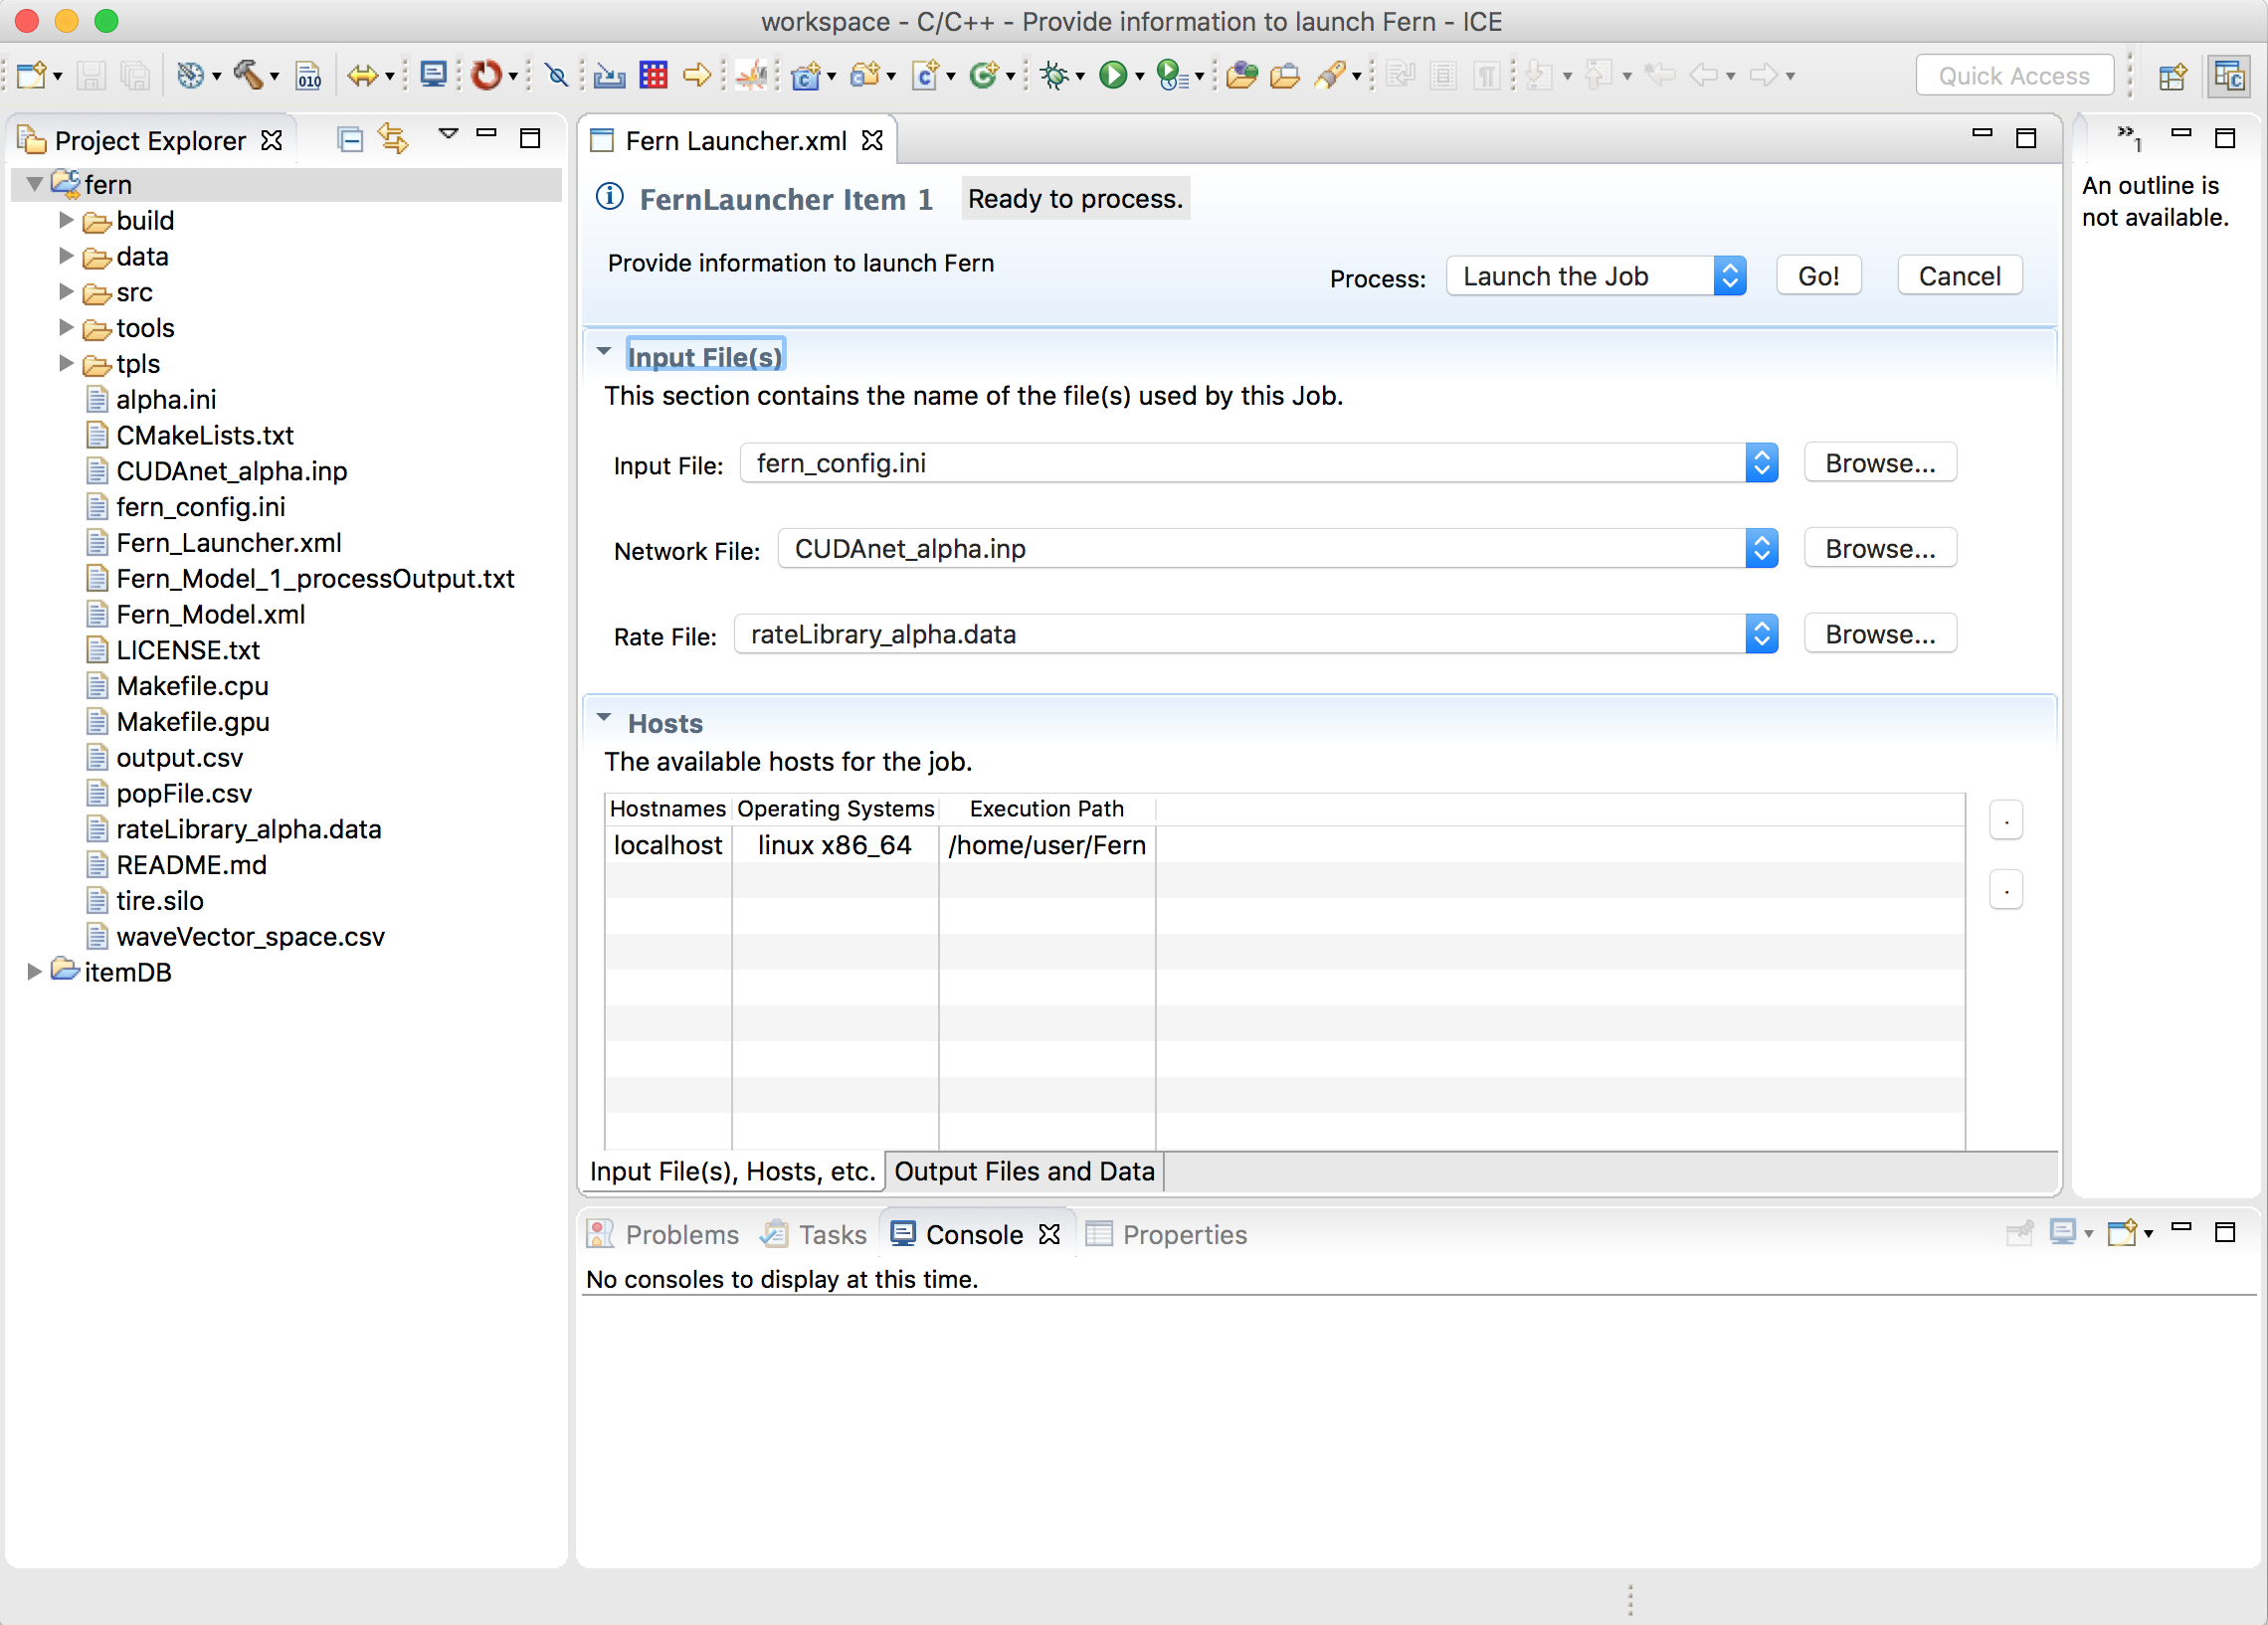
\includegraphics[width=\textwidth]{figures/launcher}
\end{center}
To configure a launch, simply set the correct
input file, along with its dependent network and rate files. 

At this point, if you had Fern built on your local machine, or if you had it
built on some remote host, you could configure that in the Hosts table. ICE
would then execute Fern based on that input. Since, for the purposes of this
tutorial, we don't have either of those configurations, we can use a third mode
of execution - launching our application via Docker. To do so, check the Launch
with Docker button, which will show a drop down widget populated with the list
of locally available Docker images. Select the eclipseice/fern image, and make
sure that the host table is configured to localhost and that the install path is
\texttt{/usr/bin}. Then simply launch Fern by clicking Go. This will pop up some
dialogs related to the connection of ICE to the Docker container, simply provide
a master password for Eclipse secure storage, and select yes on the known hosts
dialog. 

After the execution you should see the results in the Console, as shown below.
\begin{center} 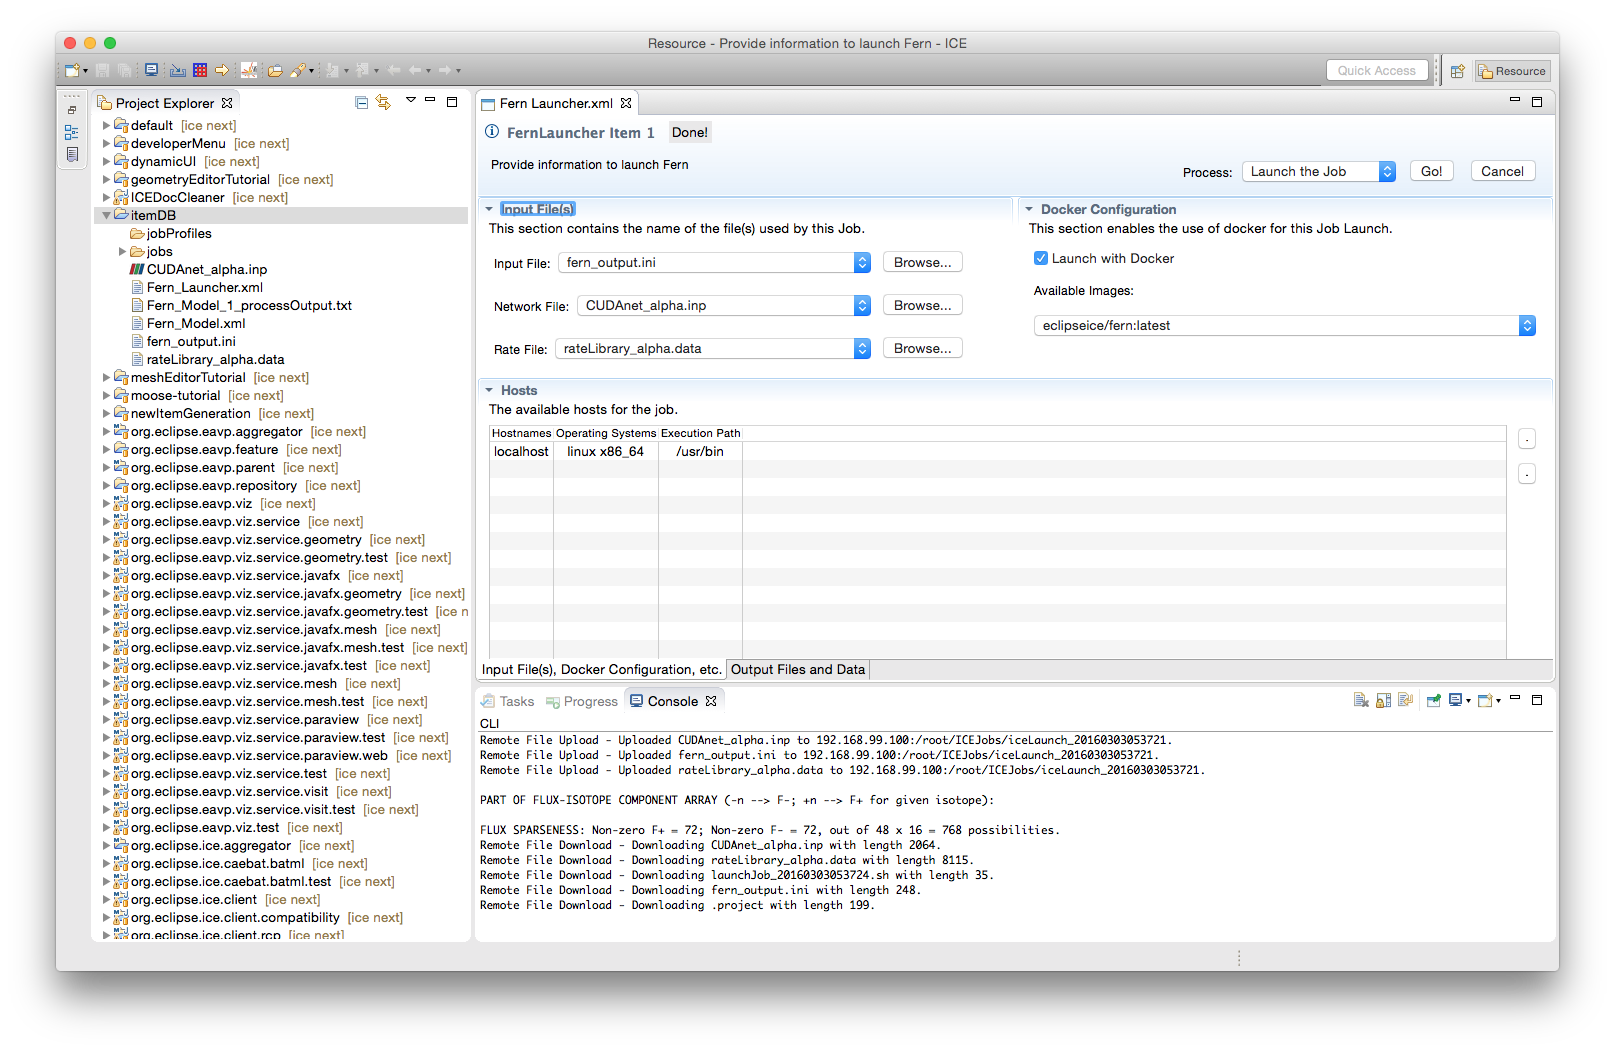
\includegraphics[width=\textwidth]{figures/launcherResult}
\end{center}
